% !TEX program = xelatex
% 编译：xelatex transformer架构.tex（建议编译两次以更新目录）
\documentclass[UTF8,a4paper,12pt]{ctexart}

\usepackage{amsmath,amssymb}
\usepackage{geometry}
\usepackage{graphicx}
\usepackage{booktabs}
\usepackage{multirow}
\usepackage{float}
\usepackage{hyperref}
\usepackage{caption}
\usepackage{enumitem}
\usepackage{xcolor}

\geometry{left=2.5cm,right=2.5cm,top=2.5cm,bottom=2.5cm}
\hypersetup{colorlinks=true,linkcolor=blue!60!black,citecolor=green!50!black,urlcolor=blue!70!black}
\graphicspath{{tier_c_project/figures/}}

\title{\textbf{深度学习基础大作业实验报告}\\[0.4em]
\large A 股趋势预测与模拟交易——档位 C Transformer 架构（TFNE-C）}
\author{
  【组员1姓名】（【学号1】）\quad
  【组员2姓名】（【学号2】）\quad
  【组员3姓名】（【学号3】）
}
\date{2026 年 5 月}

\begin{document}
\maketitle
\thispagestyle{empty}

\begin{center}
\fbox{\parbox{0.92\textwidth}{
\textbf{方案代号}：TFNE-C（TFT-lite + FT-Transformer + NewsLoRA 秩融合集成）\\
\textbf{配置}：\texttt{config.server\_c\_tfne\_72h.yaml}（72h 保证版；Top2000 / 1 seed）\\
\textbf{代码路径}：\texttt{code/}；入口 \texttt{scripts/run\_server\_c\_tfne\_72h.py}\\
\textbf{硬件}：USTC 算力平台 NVIDIA RTX 5090（31.4\,GB）；conda \texttt{ai25}\\
\textbf{作业编号}：train\_7707；完成时间 2026-05-22 20:26（UTC+8）\\
\textbf{随机种子}：42
}}
\end{center}

\begin{abstract}
本实验在档位 A 基线（RGNE-Lite）同一套数据与策略框架上，将三个子模型升级为\textbf{深度学习 Transformer 族}：时序分支采用 \textbf{TFT-lite}（双层 LSTM + 时序注意力 + 静态变量嵌入），截面分支采用 \textbf{FT-Transformer}（特征 Token 化 + 4 层自注意力），新闻分支采用 \textbf{Chinese-RoBERTa + LoRA} 微调。三模态独立训练后，经 Spearman ICIR 定权秩融合得到统一 alpha，再映射为目标权重组合并完成 T+1 历史回测。

服务器实验采用流动性 \textbf{Top 2000}、序列窗口 \textbf{60 日}、2019-01 至 2026-05 样本。融合后在验证集（2024 年下半年）全市场 mean IC 为 \textbf{0.070}、ICIR 为 \textbf{0.483}；独立测试集（2025-01 至 2026-05）mean IC 为 \textbf{0.072}、ICIR 为 \textbf{0.546}。测试集历史回测总收益 \textbf{27.3\%}、复利年化 CAGR \textbf{20.2\%}、算术年化 \textbf{20.7\%}、夏普 \textbf{0.98}、最大回撤 \textbf{-16.3\%}（330 个交易日）。验证集回测收益接近持平（总收益 \textbf{0.36\%}），说明策略在 2024 下半年样本上组合层表现一般，不宜仅依据测试段高 CAGR 外推。相对档位 A，截面 Transformer（FTT）在单模态验证 IC 与融合权重上占主导（约 61\%）。

\vspace{0.5em}
\noindent\textbf{关键词：}Transformer；TFT；FT-Transformer；LoRA；多模态融合；IC/ICIR；历史回测
\end{abstract}

\tableofcontents
\newpage

%==============================================================================
\section{任务背景与方案定位}
%==============================================================================

\subsection{作业背景与问题形式化}

与档位 A 相同，任务为\textbf{日频横截面排序}：每个交易日 $t$ 对股票池内个股 $i$ 构造特征 $X_{i,t}$，预测下一日相对沪深 300 的超额收益
\begin{equation}
  y_{i,t} = r_{i,t+1} - r^{\mathrm{mkt}}_{t+1},
\end{equation}
模型输出分数 $s_{i,t}$，主评价指标为 Spearman \textbf{IC}。策略仅在头部 quantile 选股，因此除全市场 IC 外，还报告 Top 10\% 内 IC 与多空 spread（定义同档位 A 报告）。

\subsection{档位 C 相对档位 A 的升级}

\begin{table}[H]
\centering
\caption{档位 A 基线 vs 档位 C Transformer 方案（本实验）}
\label{tab:vs-a}
\begin{tabular}{lll}
\toprule
\textbf{维度} & \textbf{档位 A（RGNE-Lite）} & \textbf{档位 C（TFNE-C，本实验）} \\
\midrule
时序模型   & GRU，$L=20$         & TFT-lite（LSTM+Attn），$L=60$ \\
截面模型   & TabMLP              & FT-Transformer（4 blocks） \\
新闻模型   & HashingVectorizer   & RoBERTa-wwm-ext + LoRA \\
股票池     & Top 500（本机）     & Top 2000（服务器） \\
数据截止   & 2024-12-31          & 2026-05-20（含独立 test） \\
随机种子   & 42                  & 42（72h 版仅 1 seed） \\
\bottomrule
\end{tabular}
\end{table}

\subsection{本实验配置说明（72h 保证版）}

为在单次 GPU 72h 配额内稳定跑通，相对满血 \texttt{config.server\_c.yaml} 做了有意缩减（详见 \texttt{report\_notes}）：
\begin{itemize}[leftmargin=2em]
  \item \texttt{liquidity\_top\_k}: 3000 $\to$ \textbf{2000}；
  \item \texttt{seeds}: [42,123,456] $\to$ \textbf{[42]}；
  \item TFT/FTT \texttt{max\_epochs}: 30 $\to$ \textbf{8}（TFT 实际 5 epoch 早停）；
  \item News 训练子采样 \textbf{4 万} 条、\textbf{3 epoch}；文本长度 128；
  \item \texttt{amp=false}, \texttt{tf32=false}（Top 全量 TFT 数值稳定）。
\end{itemize}
在 RTX 5090 上实测 train+eval 总 GPU 时间约 \textbf{3.2 小时}，远低于 72h 上限；更高配置见 \texttt{config.server\_c\_5090\_72h.yaml}（文档 \texttt{USTC\_SUBMIT\_5090\_72H.md}）。

\subsection{产物完整性说明}

本地 \texttt{code/artifacts/tier\_c/} 已包含本次服务器实验的\textbf{评估闭环}产物：
\begin{itemize}[leftmargin=2em]
  \item \texttt{metrics/tier\_c/ic\_summary.json} — IC/ICIR/spread；
  \item \texttt{backtest/tier\_c/\{valid,test\}/} — 净值与回测指标；
  \item \texttt{predictions/tier\_c/fusion\_weights.json} — 融合权重；
  \item \texttt{orders/tier\_c/orders\_20260520.csv} — 最新调仓；
  \item \texttt{features/feature\_meta.json}、\texttt{panel\_features.parquet} — 特征面板；
  \item \texttt{checkpoints/tier\_c/\{tft,ftt,news\}/seed\_42/best.pt} — 三模态权重（News 约 410\,MB）。
\end{itemize}
服务器 prep 与训练日志位于 \texttt{/home/scc/pb23151824/pro/code/artifacts/}；\textbf{本机已同步 checkpoint 与评估产物}，可直接做增量预测（流程见第~\ref{sec:predict-update} 节）。目录中仍保留档位 A、smoke 的旧结果，\textbf{勿与 tier\_c 混淆}。

%==============================================================================
\section{数据处理与特征工程}
%==============================================================================

数据处理流水线与档位 A 相同（\texttt{01\_build\_panel.py} $\to$ \texttt{02\_make\_features.py} $\to$ \texttt{02b\_embed\_news.py}），仅规模与窗口不同。防泄露规则（逐日截面 winsorize+rank、新闻 T+1 映射、按日期切分）见档位 A 报告表~\ref{tab:leak-check}，此处不重复。

\begin{table}[H]
\centering
\caption{本实验数据划分（来自 \texttt{ic\_summary.json} 有效天数）}
\label{tab:split-c}
\begin{tabular}{lcll}
\toprule
\textbf{集合} & \textbf{截止规则} & \textbf{IC 天数} & \textbf{用途} \\
\midrule
训练集 & $\le$ 2024-06-30 & 1327 & 三模态训练 \\
验证集 & 2024-07-01 --- 2024-12-31 & 125 & IC 评估 + 融合定权 + 回测 \\
测试集 & $>$ 2024-12-31 & 330 & 样本外 IC + 回测（至 2026-05） \\
\bottomrule
\end{tabular}
\end{table}

\begin{table}[H]
\centering
\caption{特征配置（\texttt{feature\_meta.json}）}
\label{tab:feat}
\begin{tabular}{ll}
\toprule
\textbf{类型} & \textbf{列名} \\
\midrule
时序 16 维 & \texttt{ret\_*d}, \texttt{vol\_*d}, \texttt{amp}, \texttt{vwap\_dev}, \texttt{log\_amount}, 资金流, \texttt{rsi\_14} 等 \\
截面 9 维  & \texttt{turnover\_rate\_f}, \texttt{pb}, \texttt{pe\_ttm}, \texttt{log\_mv}, 资金流等 \\
序列长度   & $L=60$（档位 C 标准窗口） \\
\bottomrule
\end{tabular}
\end{table}

%==============================================================================
\section{模型设计与方法论}
%==============================================================================

\subsection{总体架构 TFNE-C}

\begin{figure}[H]
\centering
\fbox{\parbox{0.90\textwidth}{\centering
\vspace{0.8em}
\textbf{模态 A（TFT-lite）}：过去 60 日价量序列 + 静态变量 $\xrightarrow{\text{LSTM+Attn}}$ $z_A$ \\[0.4em]
\textbf{模态 B（FT-Transformer）}：当日 9 维截面因子 $\xrightarrow{\text{Self-Attn}\times 4}$ $z_B$ \\[0.4em]
\textbf{模态 C（NewsLoRA）}：当日新闻文本 $\xrightarrow{\text{RoBERTa+LoRA}}$ $z_C$ \\[0.6em]
$z_A,z_B,z_C \xrightarrow{\text{逐日截面秩 + ICIR 定权}}$ 融合 score $\xrightarrow{\text{目标权重}}$ T+1 回测 \\[0.8em]
}}
\caption{TFNE-C 总体架构示意}
\label{fig:arch-c}
\end{figure}

三模态\textbf{独立训练}、独立保存 \texttt{best.pt}，融合阶段映射为 \texttt{A/B/C}（分别对应 tft / ftt / news 预测文件）。

\subsection{模态 A：TFT-lite（时序 Transformer 风格）}

\textbf{不是 BERT}，而是 Temporal Fusion Transformer 的轻量变体（\texttt{src/models/seq\_model.py}）：
\begin{enumerate}[leftmargin=2em]
  \item 双层 \texttt{LSTM}（hidden=128）编码 $(B,60,16)$ 序列；
  \item 时序注意力对 60 步加权汇聚（padding 位置 mask）；
  \item 静态变量：行业 embedding + \texttt{log\_mv} + \texttt{listing\_age} 投影，与时序上下文拼接；
  \item MLP 头输出标量 $z_A$。
\end{enumerate}
训练验证：5 epoch 早停（patience=3），单模态最佳验证 IC $\approx$ \textbf{0.0024}，弱于 FTT。

\subsection{模态 B：FT-Transformer（表格 Transformer）}

\textbf{不是 BERT}，而是 Gorishniy 等提出的 \textbf{FT-Transformer}（\texttt{rtdl} 库，\texttt{src/models/tab\_model.py}）：
\begin{itemize}[leftmargin=2em]
  \item 每个数值特征经线性层映射为 token，共 9 个 token + 类别 token；
  \item 4 层 Transformer block（$d_{\mathrm{token}}=128$）做特征间自注意力；
  \item 从零训练，不使用 NLP 预训练权重。
\end{itemize}
训练验证：跑满 8 epoch，最佳验证 IC $\approx$ \textbf{0.0676}（epoch 7），为三模态最强。

\subsection{模态 C：NewsLoRA（BERT 族预训练 + 微调）}

\textbf{此处使用 BERT 族模型}：\texttt{hfl/chinese-roberta-wwm-ext} + LoRA（$r=8,\alpha=16$），最大长度 128。训练子采样 4 万条、3 epoch，最佳验证 IC $\approx$ \textbf{0.0261}。加载预训练权重时 \texttt{cls.predictions.*} 等 MLM 头显示 \texttt{UNEXPECTED} 为正常现象。

\subsection{训练超参数（本实验）}

\begin{table}[H]
\centering
\caption{档位 C 72h 保证版训练超参}
\label{tab:hyper-c}
\begin{tabular}{llp{5.5cm}}
\toprule
\textbf{项} & \textbf{取值} & \textbf{说明} \\
\midrule
优化器 & AdamW, $lr=3\times 10^{-4}$ & TFT/FTT \\
News $lr$ & $2\times 10^{-4}$ & LoRA 微调 \\
损失 & Huber($\delta=1.0$) & 抗极端收益 \\
batch & 4096（股-日） & RTX 5090 稳定 \\
TFT/FTT epoch & max 8, patience 3/8 & TFT 5 轮停 \\
News & 3 epoch, 4 万样本 & 子采样提速 \\
AMP / TF32 & 均关闭 & 防 TFT loss=nan \\
GPU 总耗时 & $\approx$3.2 h & 含 precompute+eval \\
\bottomrule
\end{tabular}
\end{table}

\subsection{秩融合}

与档位 A 相同：逐日对 $z_A,z_B,z_C$ 做截面秩变换，按验证集各模态 ICIR 定权（\texttt{src/ensemble.py}）。本实验融合权重为：
\begin{itemize}[leftmargin=2em]
  \item $w_A$（TFT）$\approx$ \textbf{5.5\%}；
  \item $w_B$（FTT）$\approx$ \textbf{60.7\%}；
  \item $w_C$（News）$\approx$ \textbf{33.8\%}。
\end{itemize}
FTT 主导融合，与单模态验证 IC 排序一致；News 权重大于 TFT，说明 RoBERTa-LoRA 提供增量信息。

%==============================================================================
\section{交易策略与回测设置}
%==============================================================================

策略与档位 A 相同（\texttt{src/strategy.py}）：在 score Top 10\%（\texttt{q\_min=0.90}）内 softmax 加权，最多 \texttt{n\_max=50} 只，单票上限 5\%、行业 25\%、最低现金 3\%，T+1 成交，含佣金/印花税/滑点。初始资金 100 万元。参数见 \texttt{config.server\_c\_tfne\_72h.yaml} 中 \texttt{strategy} 段。

%==============================================================================
\section{更新数据与最新策略预测}
\label{sec:predict-update}
%==============================================================================

训练完成后，模拟赛与日常调仓均\textbf{不再重训}，而是在更新 \texttt{../data/} 原始 CSV 后，沿 prep $\to$ 推理融合 $\to$ 出单 流水线生成最新 \texttt{target\_weight}。\textbf{必须固定使用训练时同一配置} \texttt{config.server\_c\_tfne\_72h.yaml}（Top2000、$L=60$、seed=42、特征列与 \texttt{feature\_meta.json} 一致），否则 checkpoint 与特征维度不匹配。

\subsection{流水线总览}

\begin{figure}[H]
\centering
\fbox{\parbox{0.92\textwidth}{\centering
\vspace{0.6em}
\textbf{../data/*.csv}（追加最新 \texttt{daily/}、\texttt{news/} 等）\\[0.3em]
$\downarrow$ \texttt{01\_build\_panel} $\to$ \texttt{02\_make\_features} $\to$ \texttt{02b\_embed\_news}（CPU）\\[0.3em]
$\downarrow$ \texttt{04\_ensemble\_predict}（GPU：TFT/FTT 读 checkpoint 全量推理 + 秩融合）\\[0.3em]
$\downarrow$ \texttt{07\_predict\_latest}（读融合 score + 策略层 $\to$ \texttt{orders\_YYYYMMDD.csv}）\\[0.6em]
}}
\caption{更新数据后的预测与调仓流水线（不重训 TFT/FTT）}
\label{fig:predict-pipe}
\end{figure}

各脚本职责见表~\ref{tab:predict-scripts}。\texttt{07\_predict\_latest.py} \textbf{不调用神经网络}：它读取 \texttt{ensemble\_scores.parquet} 中最后一个 \texttt{trade\_date} 的 score，结合当日可交易股票池与 \texttt{strategy} 参数输出目标权重。

\begin{table}[H]
\centering
\caption{预测相关脚本与输入输出}
\label{tab:predict-scripts}
\begin{tabular}{llp{5.2cm}}
\toprule
\textbf{脚本} & \textbf{主要输入} & \textbf{输出} \\
\midrule
\texttt{01\_build\_panel} & \texttt{../data/} CSV & \texttt{panel\_daily.parquet} \\
\texttt{02\_make\_features} & 面板 + GKX 变换 & \texttt{features/panel\_features.parquet} \\
\texttt{02b\_embed\_news} & 新闻 CSV + 面板 & \texttt{news/panel\_news.parquet} \\
\texttt{04\_ensemble\_predict} & 特征面板 + checkpoint & \texttt{predictions/tier\_c/ensemble\_scores.parquet} \\
\texttt{03\_train\_news\_lora} & 特征 + 新闻（可选） & \texttt{predictions/tier\_c/news/seed\_42.parquet} \\
\texttt{07\_predict\_latest} & 融合 score + 面板 & \texttt{orders/tier\_c/orders\_*.csv} \\
\bottomrule
\end{tabular}
\end{table}

\subsection{三种使用场景}

\begin{table}[H]
\centering
\caption{更新数据后的三种操作路径}
\label{tab:predict-scenarios}
\begin{tabular}{p{3.2cm}p{4.2cm}p{5.8cm}}
\toprule
\textbf{场景} & \textbf{何时使用} & \textbf{命令} \\
\midrule
A.\ 仅出单 & \texttt{../data/} 未变；\texttt{ensemble\_scores} 已含最新日 & 只跑 \texttt{07\_predict\_latest.py} \\
B.\ 新交易日 & \texttt{daily/} 等 CSV 有新日期，需扩展 score & prep（01--02b）$\to$ \texttt{04} $\to$ \texttt{07} \\
C.\ 完整三模态 & 新日期且需 News 模态完整参与融合 & B + 重跑 \texttt{03\_train\_news\_lora} 后再 \texttt{04} \\
\bottomrule
\end{tabular}
\end{table}

\textbf{场景 A} 适用于本实验已跑完 eval、面板与融合 score 均截止 \textbf{2026-05-20} 的情况：直接生成 \texttt{orders\_20260520.csv} 即可下单。

\textbf{场景 B/C} 适用于模拟赛每日收盘后：将新行情 CSV 放入 \texttt{../data/} 对应目录后，按下列命令刷新 score 与订单（在 \texttt{code/} 目录、conda \texttt{ai25} 下执行）。

\subsection{本机命令（Windows PowerShell）}

\paragraph{（1）场景 A：数据未变，仅刷新调仓 CSV}

\begin{verbatim}
conda activate ai25
cd code
python scripts/07_predict_latest.py --config config.server_c_tfne_72h.yaml
\end{verbatim}

输出：\texttt{artifacts/orders/tier\_c/orders\_<最后交易日>.csv}。

\paragraph{（2）场景 B：CSV 有新日期，扩展融合 score}

\begin{verbatim}
conda activate ai25
cd code
python scripts/01_build_panel.py --config config.server_c_tfne_72h.yaml
python scripts/02_make_features.py --config config.server_c_tfne_72h.yaml
python scripts/02b_embed_news.py --config config.server_c_tfne_72h.yaml
python scripts/04_ensemble_predict.py --config config.server_c_tfne_72h.yaml
python scripts/07_predict_latest.py --config config.server_c_tfne_72h.yaml
\end{verbatim}

\texttt{04\_ensemble\_predict.py} 对 TFT/FTT 从 \texttt{checkpoints/tier\_c/} 加载 \texttt{best.pt}，对\textbf{整个} \texttt{panel\_features.parquet} 推理；融合权重默认读取 \texttt{fusion\_weights.json}（本实验 $w_A\!\approx\!5.5\%$, $w_B\!\approx\!60.7\%$, $w_C\!\approx\!33.8\%$），\textbf{无需在验证集上重新定权}，除非刻意删除该文件令脚本重估。

\paragraph{（3）场景 C：新日期需 News 模态完整覆盖}

\texttt{04} 对新闻分支\textbf{不会}从 checkpoint 自动推理新日期，而是读取已有 \texttt{predictions/tier\_c/news/seed\_42.parquet}。若 prep 后出现了该文件未覆盖的新 \texttt{trade\_date}，News 秩为缺失，融合 score 退化为 mainly TFT+FTT（约 66\% 权重仍有效，但不完整）。要恢复三模态，在 \texttt{04} 之前追加：

\begin{verbatim}
$env:HF_ENDPOINT = "https://hf-mirror.com"
python scripts/03_train_news_lora.py --config config.server_c_tfne_72h.yaml --seed 42
python scripts/04_ensemble_predict.py --config config.server_c_tfne_72h.yaml
python scripts/07_predict_latest.py --config config.server_c_tfne_72h.yaml
\end{verbatim}

注意：\texttt{03\_train\_news\_lora.py} 会\textbf{重新训练} LoRA 并写回 \texttt{news/seed\_42.parquet}（耗时与 GPU 显存占用显著高于 TFT/FTT 推理）。模拟赛若时间紧，可暂用场景 B，仅在 News 缺失日占比高时再跑场景 C。

\subsection{从 score 到模拟下单}

与档位 A 相同，操作映射为：
\begin{enumerate}[leftmargin=2em]
  \item 每个交易日 \textbf{T 收盘后}，确保 \texttt{../data/} 已更新至 \textbf{T}（策略使用 T 日特征预测 T+1 超额，无未来信息）；
  \item 按场景 A/B/C 运行脚本，读取 \texttt{orders\_YYYYMMDD.csv} 中 \texttt{ts\_code} 与 \texttt{target\_weight}；
  \item 目标市值 $=$ 账户总资产 $\times$ \texttt{target\_weight}，与当前持仓 diff 得买卖清单；
  \item \textbf{T+1} 交易时段委托；遵守涨停/停牌/T+1 可卖与尽可能满仓规则。
\end{enumerate}

\subsection{注意事项}

\begin{itemize}[leftmargin=2em]
  \item \textbf{配置不可混用}：勿用 \texttt{smoke\_c}、\texttt{tier\_a} 等 config 加载 \texttt{tier\_c} checkpoint；\texttt{tier\_tag()} 不同会导致路径错位。
  \item \textbf{GPU 建议}：TFT/FTT 推理 Top2000 全历史可在 GPU 上数分钟内完成；NewsLoRA 强烈建议 GPU（checkpoint $\approx$410\,MB）。
  \item \textbf{依赖}：\texttt{requirements.txt} + \texttt{requirements-nlp.txt}（\texttt{transformers}、\texttt{peft}、\texttt{rtdl}）。
  \item \textbf{缺失模态}：某日某股无新闻时，\texttt{rank\_C} 为 NaN，融合时该模态不参与加权（见 \texttt{src/ensemble.py}），score 仍可由 TFT/FTT 给出。
  \item \textbf{换股票池或改 $L$}：需按新配置重新 prep + 全量训练，不能直接复用本次 checkpoint。
\end{itemize}

%==============================================================================
\section{评价指标定义}
%==============================================================================

IC、ICIR、Top 分位 IC、多空 spread、CAGR、算术年化、Sharpe、MDD 的定义与档位 A 报告第 5 节一致（$r_f=0$，年化 252 日）。实现：\texttt{src/metrics.py}、\texttt{src/backtest.py}。

\textbf{读数提醒：} spread 年化 $\approx \overline{\mathrm{spread}}\times 252$ 为\textbf{未扣费、多空对称}参考；组合回测经仓位约束与成本，通常低于 spread 暗示的上限。

%==============================================================================
\section{实验结果与对比分析}
%==============================================================================

\subsection{预测能力：IC / ICIR / Spread}

\begin{table}[H]
\centering
\caption{验证集预测指标（2024-07-01 --- 2024-12-31，融合 score）}
\label{tab:ic-valid}
\begin{tabular}{lcccc}
\toprule
\textbf{指标} & \textbf{mean IC / spread} & \textbf{std} & \textbf{ICIR / 年化} & \textbf{天数} \\
\midrule
全市场 IC     & 0.0701 & 0.145 & 0.483 & 125 \\
Top 10\% 内 IC & 0.0051 & 0.116 & 0.044 & 125 \\
多空 spread（日） & 0.382\% & 1.43\% & 年化 96.3\% & 125 \\
\bottomrule
\end{tabular}
\end{table}

\begin{table}[H]
\centering
\caption{测试集预测指标（2025-01-01 起，330 日，样本外）}
\label{tab:ic-test}
\begin{tabular}{lcccc}
\toprule
\textbf{指标} & \textbf{mean IC / spread} & \textbf{std} & \textbf{ICIR / 年化} & \textbf{天数} \\
\midrule
全市场 IC     & 0.0715 & 0.131 & 0.546 & 330 \\
Top 10\% 内 IC & 0.0062 & 0.104 & 0.060 & 330 \\
多空 spread（日） & 0.310\% & 1.15\% & 年化 78.1\% & 330 \\
\bottomrule
\end{tabular}
\end{table}

\begin{table}[H]
\centering
\caption{训练集预测指标（对照，融合 score）}
\label{tab:ic-train}
\begin{tabular}{lcccc}
\toprule
\textbf{指标} & \textbf{mean IC / spread} & \textbf{std} & \textbf{ICIR / 年化} & \textbf{天数} \\
\midrule
全市场 IC     & 0.0687 & 0.111 & 0.619 & 1327 \\
Top 10\% 内 IC & 0.0089 & 0.101 & 0.089 & 1327 \\
多空 spread（日） & 0.379\% & 1.12\% & 年化 95.4\% & 1327 \\
\bottomrule
\end{tabular}
\end{table}

\textbf{解读：}
\begin{itemize}[leftmargin=2em]
  \item 融合后全市场 IC $\approx 0.07$，显著高于档位 A 验证集 0.026，主要得益于 Top2000 规模、60 日窗口与 FTT/News Transformer 模态；
  \item 验证/测试 IC 接近且测试 ICIR 略高，样本外排序能力未明显崩塌；
  \item Top 10\% 内 IC 仍接近 0（0.005--0.006）：头部内部细分仍难，但 spread 显著为正，策略逻辑仍成立；
  \item 单模态训练 IC（TFT 0.0024 vs FTT 0.0676）与融合权重一致：截面 Transformer 是核心 alpha 来源。
\end{itemize}

\begin{figure}[H]
\centering

\includegraphics[width=0.82\textwidth]{fig2_ic_summary.png}
\caption{训练 / 验证 / 测试集 IC 与 ICIR 对比（融合 score）}
\label{fig:ic-bar}
\end{figure}

\begin{figure}[H]
\centering

\includegraphics[width=\textwidth]{fig5_ic_timeseries.png}
\caption{日度 Spearman IC 及 20 日滚动均值（虚线：验证集 2024-07-01、测试集 2025-01-01 起点）}
\label{fig:ic-ts}
\end{figure}

\subsection{历史回测}

\begin{table}[H]
\centering
\caption{验证集历史回测（2024-07-01 --- 2024-12-31，124 个交易日）}
\label{tab:bt-valid}
\begin{tabular}{lr}
\toprule
\textbf{指标} & \textbf{本策略} \\
\midrule
总收益率 $R_{\mathrm{tot}}$     & 0.36\% \\
复利年化 CAGR  & 0.73\% \\
算术年化收益   & 6.14\% \\
年化波动率     & 32.92\% \\
夏普比率       & 0.19 \\
最大回撤 MDD   & -16.54\% \\
期末净值       & 100.36 万元 \\
\bottomrule
\end{tabular}
\end{table}

\begin{table}[H]
\centering
\caption{测试集历史回测（330 个交易日，2025-01 起）}
\label{tab:bt-test}
\begin{tabular}{lr}
\toprule
\textbf{指标} & \textbf{本策略} \\
\midrule
总收益率 $R_{\mathrm{tot}}$     & \textbf{27.26\%} \\
复利年化 CAGR  & \textbf{20.21\%} \\
算术年化收益   & \textbf{20.71\%} \\
年化波动率     & 21.17\% \\
夏普比率       & \textbf{0.98} \\
最大回撤 MDD   & -16.26\% \\
期末净值       & 127.26 万元 \\
\bottomrule
\end{tabular}
\end{table}

\textbf{解读：} 验证集组合层几乎不赚钱（总收益 0.36\%），与 IC/spread 看似矛盾，可能原因包括：2024 下半年市场环境、换手与成本、Top2000 与策略参数未针对该段调优。\textbf{测试段表现较好不应直接外推}，需在报告中同时呈现验证段与测试段，并说明样本长度差异（125 vs 330 日）。

\begin{figure}[H]
\centering
\begin{minipage}{0.48\textwidth}
  \centering
  
\includegraphics[width=\textwidth]{fig1_valid_equity.png}
  \caption{验证集净值（2024H2）}
  \label{fig:eq-valid}
\end{minipage}\hfill
\begin{minipage}{0.48\textwidth}
  \centering
  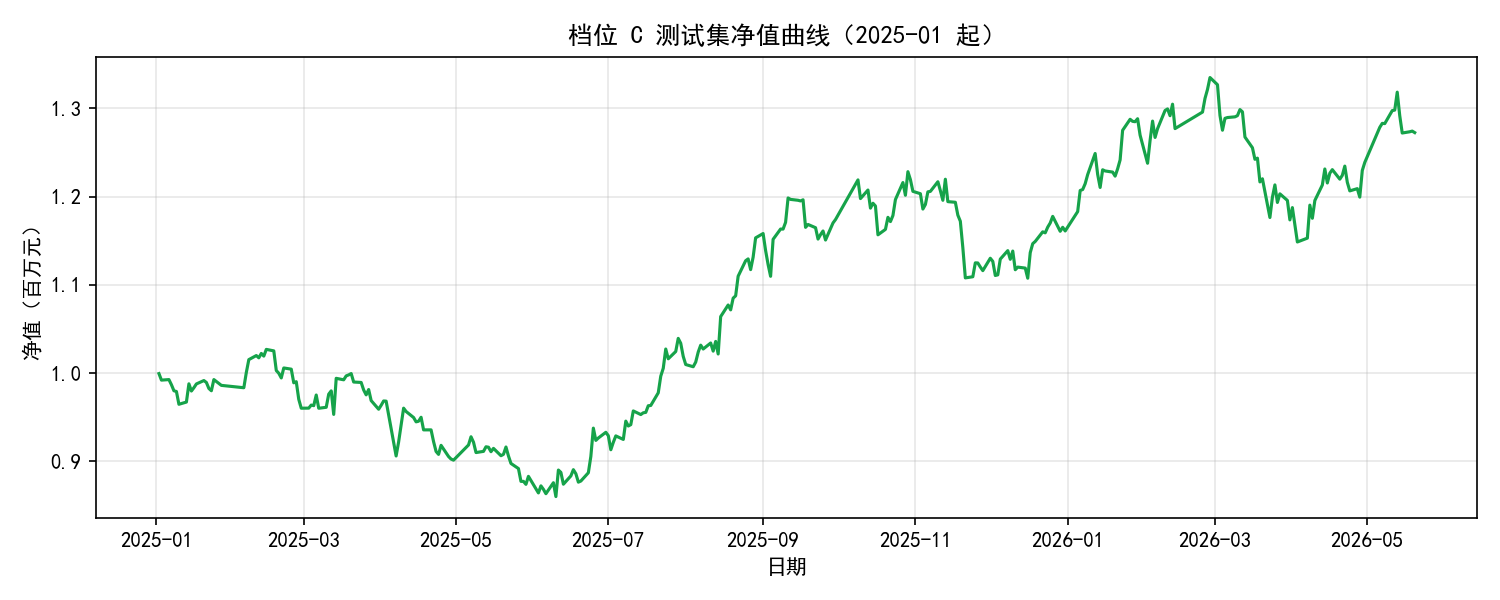
\includegraphics[width=\textwidth]{fig1_test_equity.png}
  \caption{测试集净值（2025 起）}
  \label{fig:eq-test}
\end{minipage}
\end{figure}

\subsection{融合权重与最新调仓}

\begin{table}[H]
\centering
\caption{验证集 ICIR 融合权重（\texttt{fusion\_weights.json}）}
\label{tab:fusion}
\begin{tabular}{llr}
\toprule
\textbf{代号} & \textbf{模型} & \textbf{权重} \\
\midrule
A & TFT-lite   & 5.53\% \\
B & FT-Transformer & 60.71\% \\
C & NewsLoRA   & 33.77\% \\
\bottomrule
\end{tabular}
\end{table}

\begin{figure}[H]
\centering
\begin{minipage}{0.46\textwidth}
  \centering
  
\includegraphics[width=\textwidth]{fig3_fusion_weights.png}
  \caption{三模态 ICIR 融合权重}
  \label{fig:fusion}
\end{minipage}\hfill
\begin{minipage}{0.52\textwidth}
  \centering
  
\includegraphics[width=\textwidth]{fig4_latest_orders.png}
  \caption{最新调仓 Top15 目标权重（2026-05-20）}
  \label{fig:orders}
\end{minipage}
\end{figure}

最新调仓文件：\texttt{artifacts/orders/tier\_c/orders\_20260520.csv}（trade\_date=20260520，最多 50 只目标权重）。模拟赛每日更新数据后的完整预测流程见第~\ref{sec:predict-update} 节；若仅复用已有融合 score，收盘后运行 \texttt{07\_predict\_latest.py} 即可，次日按 \texttt{target\_weight} 下单。

\subsection{相对档位 A 的简要对比}

\begin{table}[H]
\centering
\caption{档位 A 基线 vs 档位 C 本实验（验证集）}
\label{tab:cmp-a}
\begin{tabular}{lcc}
\toprule
\textbf{指标} & \textbf{档位 A} & \textbf{档位 C（本实验）} \\
\midrule
股票池 & Top 500 & Top 2000 \\
全市场 mean IC & 0.026 & \textbf{0.070} \\
ICIR & 0.195 & \textbf{0.483} \\
验证集总收益 & 26.0\% & 0.36\% \\
验证集 Sharpe & 1.41 & 0.19 \\
\bottomrule
\end{tabular}
\end{table}

\textbf{注意：} 两档实验股票池、时间覆盖、模型复杂度不同，\textbf{不宜仅凭 IC 升高断定组合一定更好}。本实验测试段回测较优，验证段回测偏弱，说明 Transformer 升级主要改善\textbf{排序指标}，组合层仍依赖市场环境与策略参数。

%==============================================================================
\section{规范性与可复现性}
%==============================================================================

\begin{table}[H]
\centering
\caption{复现命令（服务器训练 + 本机增量预测）}
\label{tab:repro}
\begin{tabular}{p{11cm}}
\toprule
\textbf{步骤} \\
\midrule
\texttt{sbatch scripts/slurm\_prep\_cpu\_tfne\_72h.sbatch} \\
\texttt{sbatch scripts/slurm\_train\_gpu\_tfne\_72h.sbatch} \\
或 \texttt{python scripts/run\_server\_c\_tfne\_72h.py train \&\& ... eval} \\
配置固定为 \texttt{config.server\_c\_tfne\_72h.yaml}，seed=42 \\
\midrule
\textbf{本机更新数据后预测（不重训）}：见第~\ref{sec:predict-update} 节；\\
\texttt{04\_ensemble\_predict.py} + \texttt{07\_predict\_latest.py} \\
\bottomrule
\end{tabular}
\end{table}

\begin{itemize}[leftmargin=2em]
  \item 训练前修复 \texttt{src/dataset.py} 静态特征 NaN 问题（\texttt{listing\_age}/\texttt{log\_mv}）；
  \item 预检 \texttt{src/preflight.py}：NaN 列仅 WARN，不阻断 train；
  \item 作业日志：\texttt{logs/train\_7707.out}。
\end{itemize}

%==============================================================================
\section{总结与反思}
%==============================================================================

\subsection{主要结论}

\begin{enumerate}[leftmargin=2em]
  \item TFNE-C 在 RTX 5090 上约 3.2 小时完成 Top2000 三模态 train+eval，工程可行；
  \item FT-Transformer 截面模态显著强于 TFT-lite 时序模态，融合权重约 61\%；
  \item NewsLoRA 贡献约 34\% 权重，验证 RoBERTa 微调优于档位 A 哈希新闻；
  \item 融合 IC 约 0.07、测试段 Sharpe 约 0.98，但验证段组合收益接近 0，报告需分段表述。
\end{enumerate}

\subsection{局限与后续工作}

\begin{itemize}[leftmargin=2em]
  \item 72h 版仅 1 个 seed，满血三 seed 见 \texttt{config.server\_c\_5090\_72h.yaml}；
  \item Top2000 而非 Top3000；News 训练子采样 4 万条；
  \item TFT 单模态 IC 仍低，可尝试更长训练或改进时序架构；
  \item 验证段回测弱，需结合基准对比与参数敏感性分析；
  \item FDL2026 模拟交易结果待赛后补充。
\end{itemize}

\section*{参考文献}
\addcontentsline{toc}{section}{参考文献}
\begin{enumerate}[leftmargin=2em]
  \item Gu, S., Kelly, B., \& Xiu, D. (2020). Empirical Asset Pricing via Machine Learning. \textit{Review of Financial Studies}.
  \item Gorishniy, Y., et al. (2021). Revisiting Deep Learning Models for Tabular Data. \textit{NeurIPS} (FT-Transformer).
  \item Lim, B., et al. (2021). Temporal Fusion Transformers for Interpretable Multi-horizon Time Series Forecasting.
  \item Hu, E. J., et al. (2021). LoRA: Low-Rank Adaptation of Large Language Models.
\end{enumerate}

\section{主要产物路径}
\addcontentsline{toc}{section}{主要产物路径}

\begin{table}[H]
\centering
\small
\begin{tabular}{ll}
\toprule
\textbf{内容} & \textbf{路径（tier\_c）} \\
\midrule
IC 汇总 & \texttt{code/artifacts/metrics/tier\_c/ic\_summary.json} \\
融合权重 & \texttt{code/artifacts/predictions/tier\_c/fusion\_weights.json} \\
融合 score & \texttt{code/artifacts/predictions/tier\_c/ensemble\_scores.parquet} \\
回测指标 & \texttt{code/artifacts/backtest/tier\_c/\{valid,test\}/metrics.json} \\
净值曲线 & \texttt{code/artifacts/backtest/tier\_c/\{valid,test\}/equity\_curve.csv} \\
最新订单 & \texttt{code/artifacts/orders/tier\_c/orders\_20260520.csv} \\
模型 checkpoint & \texttt{code/artifacts/checkpoints/tier\_c/\{tft,ftt,news\}/seed\_42/best.pt} \\
\bottomrule
\end{tabular}
\end{table}

\end{document}
